\documentclass[12pt]{extarticle}
\usepackage[english,ukrainian]{babel}
\usepackage[utf8]{inputenc}
\usepackage{amsmath,amssymb}
\usepackage{parskip}
\usepackage{graphicx}
\usepackage{xcolor}
\usepackage{tcolorbox}
\tcbuselibrary{skins}
\usepackage[framemethod=tikz]{mdframed}
\usepackage{chngcntr}
\usepackage{enumitem}
\usepackage{hyperref}
\usepackage{float}
\usepackage{subfig}
\usepackage{esint}
\usepackage[top=2.5cm, left=3cm, right=3cm, bottom=4.0cm]{geometry}
\usepackage[table]{xcolor}
\usepackage{algorithm}
\usepackage{algpseudocode}
\usepackage{listings}

\title{Домашня робота з курсу ``Теоретична механіка''}
\author{Студента 3 курсу групи МП-31 Захарова Дмитра}
\date{\today}

\begin{document}

\maketitle

\section*{Завдання 6}

\textbf{Випадок 1.} Спочатку розглянемо випадок, коли $OA$ направлено праворуч (див. рис. \ref{fig:1}).

\begin{figure}[H]
    \centering
    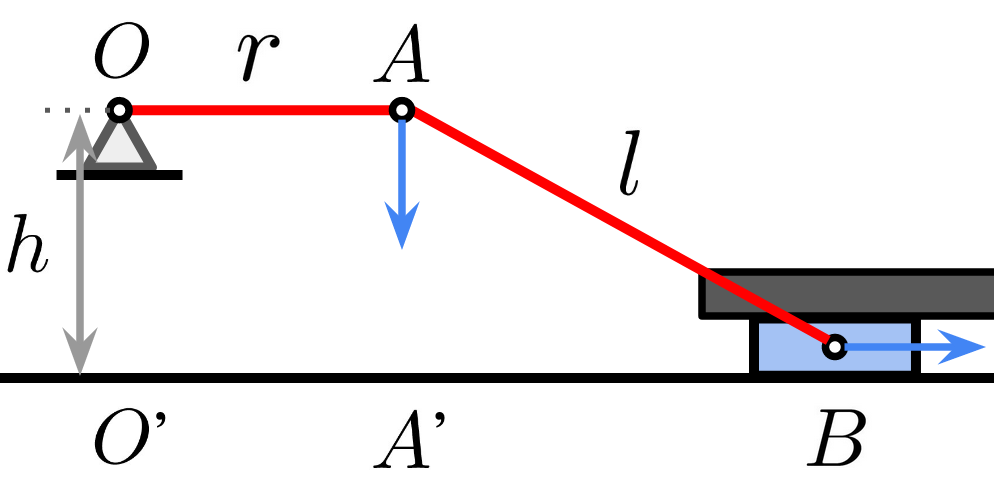
\includegraphics[width=0.6\textwidth]{images/hw_3/hw_3_1.png}
    \caption{Випадок з $OA$ направленим праворуч. $O'$ та $A'$ є проекціями на горизонталь, вздовж якої рухається грузик}
    \label{fig:1}
\end{figure}
\vspace{5px}

Швидкість точки $A$ дорівнює $v_A=\omega r$ і в цьому випадку направлена вниз (будемо вважати, що $OA$ рухається за годинниковою стрілкою). Швидкість точки $B$ направлена праворуч та нехай дорівнює $v_B$. 

Оскільки $AB$ не деформується, то проєкції $v_A$ та $v_B$ на $AB$ однакові, інакшими словами $(\boldsymbol{v}_A)_{AB} = (\boldsymbol{v}_B)_{AB}$.

Нехай кут $ABA'$ дорівнює $\theta$. Тоді $(\boldsymbol{v}_A)_{AB} = v_A \sin \theta$, а $(\boldsymbol{v}_B)_{AB} = v_B \cos \theta$. Звідси отримуємо, що $v_B = v_A \tan \theta$. З малюнку $\tan\theta = \frac{h}{\sqrt{l^2-h^2}} = \frac{1}{\sqrt{(l/h)^2-1}}$. Таким чином:
\[
v_B = \frac{\omega r}{\sqrt{l^2/h^2-1}}
\]

\textbf{Випадок 2.} Нехай $OA$ направлено вертикально вгору (див. рис. \ref{fig:2}).

\begin{figure}[H]
    \centering
    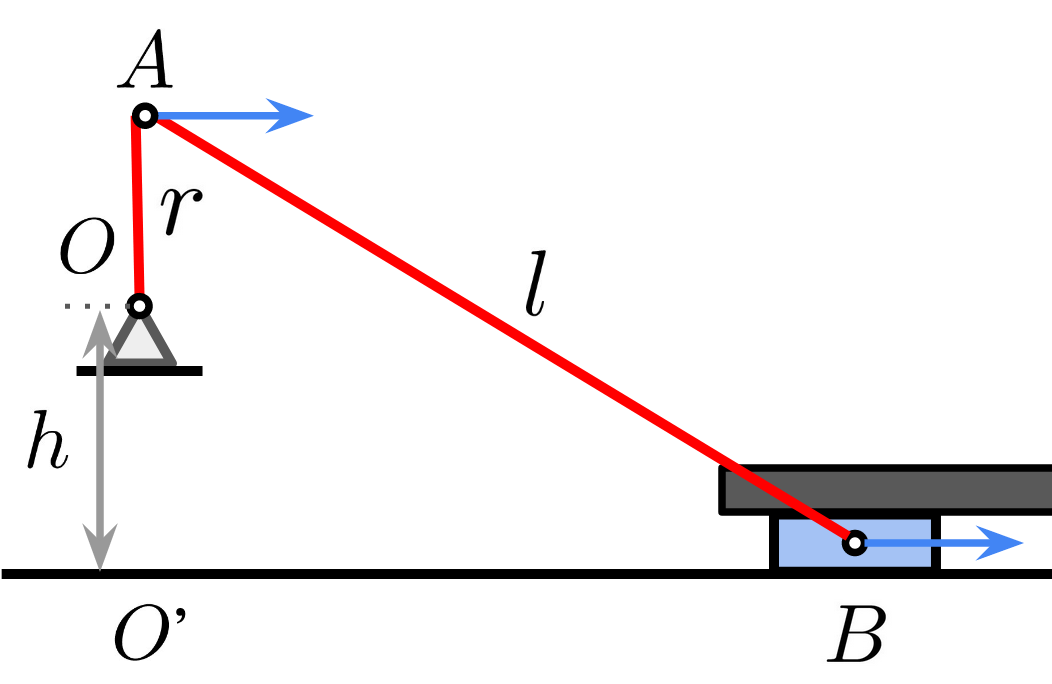
\includegraphics[width=0.5\textwidth]{images/hw_3/hw_3_2.png}
    \caption{Випадок з $OA$ направленим вгору.}
    \label{fig:2}
\end{figure}
\vspace{5px}

Оскільки $\boldsymbol{v}_A$ паралельно $\boldsymbol{v}_B$, то ці вектори складають однакові кути з $AB$. Значить, щоб проєкції були рівними, рівними мають бути модулі. Отже $v_B=v_A=\omega r$.

\textbf{Випадок 3.} Нехай $OA$ направлено ліворуч (див. рис. \ref{fig:3}).

\begin{figure}[H]
    \centering
    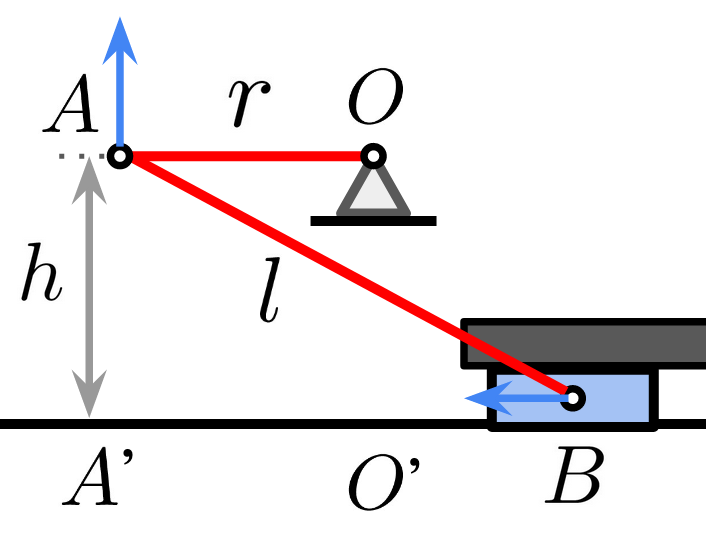
\includegraphics[width=0.5\textwidth]{images/hw_3/hw_3_3.png}
    \caption{Випадок з $OA$ направленим ліворуч. $A'$ та $O'$ є проєкціями $A,O$ на горизонтальну площину, вздовж якої рухається грузик.}
    \label{fig:3}
\end{figure}
\vspace{5px}

Знову $v_A=\omega r$ і направлено вгору. Нехай кут $BA'A$ дорівнює $\theta$. В такому разі $(\boldsymbol{v}_B)_{AB} = v_B \cos \theta$, а $(\boldsymbol{v}_A)_{AB} = v_A \sin \theta$. Тому $v_B = v_A \tan \theta$. З малюнку видно, що $\tan\theta = \frac{h}{\sqrt{l^2-h^2}} = \frac{1}{\sqrt{l^2/h^2-1}}$. Таким чином отримуємо результат, аналогічний \textit{випадку 1}.

\textbf{Відповідь.} У вертикальному положені швидкість є $\omega r$, а у горизонтальних $\frac{\omega r}{\sqrt{l^2/h^2-1}}$.

\end{document}

